%!TEX TS-program = xelatex
\documentclass[]{friggeri-cv}
\usepackage{afterpage}
\usepackage{hyperref}
\usepackage{color}
\usepackage{xcolor}
\usepackage{smartdiagram}
\usepackage{fontspec}
% if you want to add fontawesome package
% you need to compile the tex file with LuaLaTeX
% References:
%   http://texdoc.net/texmf-dist/doc/latex/fontawesome/fontawesome.pdf
%   https://www.ctan.org/tex-archive/fonts/fontawesome?lang=en
%\usepackage{fontawesome}
\usepackage{metalogo}
\usepackage{dtklogos}
\usepackage[utf8]{inputenc}
\usepackage{tikz}
\usetikzlibrary{mindmap,shadows}
\hypersetup{
    pdftitle={},
    pdfauthor={},
    pdfsubject={},
    pdfkeywords={},
    colorlinks=false,           % no lik border color
    allbordercolors=white       % white border color for all
}
\smartdiagramset{
    bubble center node font = \footnotesize,
    bubble node font = \footnotesize,
    % specifies the minimum size of the bubble center node
    bubble center node size = 0.5cm,
    %  specifies the minimum size of the bubbles
    bubble node size = 0.5cm,
    % specifies which is the distance among the bubble center node and the other bubbles
    distance center/other bubbles = 0.3cm,
    % sets the distance from the text to the border of the bubble center node
    distance text center bubble = 0.5cm,
    % set center bubble color
    bubble center node color = pblue,
    % define the list of colors usable in the diagram
    set color list = {materialgreen, green, blue, materialcyan, pblue, orange, materialteal, materialamber, materialindigo, materialgreen, materiallime},
    % sets the opacity at which the bubbles are shown
    bubble fill opacity = 0.6,
    % sets the opacity at which the bubble text is shown
    bubble text opacity = 0.5,
	priority arrow width=1cm,
	priority arrow height advance=2.25cm,
	description text width=1.7cm,
	description width = 2.1cm
}

\addbibresource{bibliography.bib}
\RequirePackage{xcolor}
\definecolor{pblue}{HTML}{0395DE}

\newcommand{\mycbox}[1]{\tikz{\path[draw=#1,fill=#1] (0,0) rectangle (0.2cm,0.3cm);}}
\newcommand{\mybbox}[1]{\tikz{\path[draw=#1,fill=#1] (0,0) rectangle (0.2cm,0.25cm);}}
\newcommand{\mydbox}[1]{\tikz{\path[draw=black,fill=#1] (0,0) rectangle (0.2cm,0.1cm);}}

\begin{document}
\header{Keith}{Wakeham}
      {M.Eng, B.Eng, Product Engineering Manager}
      
% Fake text to add separator      
\fcolorbox{white}{gray}{\parbox{\dimexpr\textwidth-2\fboxsep-2\fboxrule}{%
.....
}}

% In the aside, each new line forces a line break
\begin{aside}
%  
\includegraphics[scale=0.18]{img/snow_circle.png}
  \section{Address}
    Calgary, AB, CAN
    Vicenza, VI, IT
    ~
  \section{Tel}
    1-587-576-4142 (CAN)
    +39-347-849-3656 (IT)
    ~
  \section{Mail}
    \href{mailto:kwakeham@gmail.com}{\textbf{kwakeham@}\\gmail.com}
    ~
  \section{Web}
%    \href{http://www.keithhack.blogspot.com}{keithhack.blogspot.com}
    \href{http://ca.linkedin.com/in/kwakeham}{linkedin://kwakeham}
    \href{https://github.com/mygit}{github.com/mygit}
    ~
\section{Design}
\textbf{Mech} \mybbox{blue} $\&$ \textbf{Elec}\mybbox{materialindigo}
\href{http://www.solidworks.com/}{Solidworks} \mybbox{blue}\mybbox{blue}\mybbox{blue}\mybbox{blue}\mybbox{lightgray}
\href{http://www.altium.com/}{Altium} \mybbox{materialindigo}\mybbox{materialindigo}\mybbox{materialindigo}\mybbox{materialindigo}\mybbox{lightgray}
\href{http://kicad-pcb.org/}{Kicad} \mybbox{materialindigo}\mybbox{materialindigo}\mybbox{materialindigo}\mybbox{lightgray}\mybbox{lightgray}
\href{https://www.autodesk.com/products/eagle/overview}{Eagle} \mybbox{materialindigo}\mybbox{materialindigo}\mybbox{materialindigo}\mybbox{lightgray}\mybbox{lightgray}
\href{https://www.ptc.com/en/products/cad/pro-engineer}{PRO/E} \mybbox{blue}\mybbox{blue}\mybbox{lightgray}\mybbox{lightgray}\mybbox{lightgray}
\href{https://www.autodesk.com/products/fusion-360/students-teachers-educators}{Fusion360} \mybbox{blue}\mybbox{blue}\mybbox{lightgray}\mybbox{lightgray}\mybbox{lightgray}
~
\section{programming}
\href{http://www.mathworks.com/products/matlab/}{Matlab} \mybbox{red}\mybbox{red}\mybbox{red}\mybbox{red}\mybbox{lightgray}
\href{http://www.mathworks.com/products/simulink/}{Simulink} \mybbox{red}\mybbox{red}\mybbox{red}\mybbox{red}\mybbox{lightgray}
\href{http://www.python.org/}{Python} \mybbox{red}\mybbox{red}\mybbox{red}\mybbox{lightgray}\mybbox{lightgray}
\href{https://www.latex-project.org/)}{\LaTeX}\mybbox{red}\mybbox{red}\mybbox{red}\mybbox{lightgray}\mybbox{lightgray}
\href{https://en.wikipedia.org/wiki/C_(programming_language)}{C / C++ / C\#} \mybbox{red}\mybbox{red}\mybbox{red}\mybbox{lightgray}\mybbox{lightgray}
\href{http://www.ni.com/labview/}{Labview} \mybbox{red}\mybbox{red}\mybbox{lightgray}\mybbox{lightgray}\mybbox{lightgray}
\section{analysis} 
\href{https://en.wikipedia.org/wiki/Design_of_experiments}{DOE} \mybbox{orange}\mybbox{orange}\mybbox{orange}\mybbox{orange}\mybbox{orange}
\href{https://en.wikipedia.org/wiki/Regression_analysis}{Regression} \mybbox{orange}\mybbox{orange}\mybbox{orange}\mybbox{orange}\mybbox{lightgray}
\href{https://en.wikipedia.org/wiki/Finite_element_method}{FEA} \mybbox{orange}\mybbox{orange}\mybbox{orange}\mybbox{orange}\mybbox{lightgray}
\href{https://en.wikipedia.org/wiki/Statistics}{Statistics} \mybbox{orange}\mybbox{orange}\mybbox{orange}\mybbox{lightgray}\mybbox{lightgray}
\href{https://en.wikipedia.org/wiki/Computational_fluid_dynamics}{CFD} \mybbox{orange}\mybbox{orange}\mybbox{orange}\mybbox{lightgray}\mybbox{lightgray}
\section{simulation} 
\href{http://www.ansys.com/Products/Workflow+Technology/ANSYS+Workbench+Platform}{ANSYS} \mybbox{green}\mybbox{green}\mybbox{green}\mybbox{green}\mybbox{lightgray}
\href{http://www.ansys.com/Products/Simulation+Technology/Fluid+Dynamics/Fluid+Dynamics+Products/ANSYS+CFX}{CFX} \mybbox{green}\mybbox{green}\mybbox{green}\mybbox{green}\mybbox{lightgray}
\href{https://en.wikipedia.org/wiki/SPICE}{SPICE} \mybbox{green}\mybbox{green}\mybbox{lightgray}\mybbox{lightgray}\mybbox{lightgray}
\section{mechanical}
	\href{https://en.wikipedia.org/wiki/Machining}{Machining} \mybbox{purple}\mybbox{purple}\mybbox{purple}\mybbox{lightgray}\mybbox{lightgray}
	\href{https://en.wikipedia.org/wiki/Numerical_control}{CNC} \mybbox{purple}\mybbox{purple}\mybbox{purple}\mybbox{lightgray}\mybbox{lightgray}
	\href{https://en.wikipedia.org/wiki/Mig_welding}{Welding} \mybbox{purple}\mybbox{purple}\mybbox{lightgray}\mybbox{lightgray}\mybbox{lightgray}
%\section{Concepts}
%	\href{https://en.wikipedia.org/wiki/Lean_startup}{Lean Startup}\mybbox{materialindigo}\mybbox{materialindigo}\mybbox{materialindigo}\mybbox{materialindigo}\mybbox{lightgray}
  % use  \hspace{} or \vspace{} to change bubble size, if needed
%  \section{Mechanical}
%    \smartdiagram[bubble diagram]{
%        \textbf{FEA},
%        \textbf{CFD},
%        \textbf{Solidworks},
%        \textbf{ASME CODE},
%        \textbf{PRO/E},
%        \textbf{CFX},
%        \textbf{ANSYS}
%    }
    ~
%      \section{Electrical}
%    \smartdiagram[bubble diagram]{
%        \textbf{Altium},
%        \textbf{Kicad},
%        \textbf{Eagle},
%        \textbf{SPICE},
%        \textbf{FPGA}
%    }
    ~
%  \section{Programming}
%    \smartdiagram[bubble diagram]{
%        \textbf{C/C++},
%        \textbf{Python},
%        \textbf{GCC},
%        \textbf{Matlab},
%        \textbf{Bash}
%    }
    ~
\end{aside}
~
\section{Experience}
\begin{entrylist}
  \wentry
	{08/16 - Present}
	{Product Engineering Manager}
	{\href{https://www.campagnolo.com}{Campagnolo SRL}}
	{For the die hard cyclists, \href{https://www.campagnolo.com}{Campagnolo} elicits  \href{https://www.google.ca/search?q=campagnolo+tattoo&source=lnms&tbm=isch&sa=X&ved=0ahUKEwj34N_d0MreAhVqqVQKHd3IDLQQ_AUIDigB&biw=1742&bih=850}{fanatical loyalty} for its cycling parts, but in recent years the market shifted from electronic equipment being a high end low volume novelty to the mid range equipment the masses use without a response for Campagnolo. I approached Campagnolo knowing they wanted improved expertise in electronics and sensing and convinced them to focus on integration techniques for combining electronics with carbon fibre. I experimented and developed processes for embedding electronic sensors to survive the rigours of extreme molding pressures to create smart parts without changing visible appearance. Leading a team to explore these challenges has resulted in a new product in a new segment to be released spring 2019 utilizing these new proprietary processes.}
	{
\includegraphics[scale=0.050]{img/campa_logo.jpg} }

  \wentry
    {01/14 - 04/16}
    {Director Of Power Meter Technologies}
    {\href{https://www.4iiii.com}{4iiii Innovations Inc.}}
    {Even a startup with experienced founders can struggle to find a successful idea. Developed independently, I brought my \href{http://keithhack.blogspot.com/2013/09/prelude-to-launching-beta-test.html}{prototype powermeter} into the company with the desire to change the accessibility for elite level training tools. Turning an aesthetic mechanical part into a high accuracy load cell required bold ideas and merging advanced factorial experimental methods with multiple \href{https://en.wikipedia.org/wiki/Strain_gauge}{strain sensors} to yield the \href{https://4iiii-innovations.myshopify.com/collections/power-meters/products/precision-pro-ride-ready}{4iiii's Precision Powermeter}. With the most complicated strain gage arrangement, involved calibration and highest accuracy it achieved the lowest market price.
\href{https://en.wikipedia.org/wiki/Cycling_power_meter}{Cycling powermeters} quickly became a crowded market and 4iiii's needed to differentiate itself. Market forces dictate a more emotional connection for growth through sponsorship at an elite level. New prototypes designed by myself with the help of an expert firmware developer cinched the  \href{https://4iiii.com/proteam-precision-20160107/}{sponsorship} of a world pro cycling team. The sponsorship launched in 2016 for use in races like the Tour de France by elite professionals, but more importantly lead to a \href{https://www.specialized.com/us/en/stories/power-cranks}{contract} for 100k unit sale within a year.}
	{
\includegraphics[scale=0.016]{img/4iiii_large.jpg}}

  \wentry
    {10/11 - 01/14}
    {Project Engineering / Design Engineering}
    {\href{https://www.bwxt.com/}{Babcock and Wilcox Canada LTD.}}
    {Every tech company has their crown jewel technology and for B$\&$W that is the once through steam generator. A piece of technology that operates power plants at greater efficiency by uniquely super-heating steam. I joined design engineering where I originated and verified ASME code calculations using finite element analysis for nuclear rated components. When need arose I volunteered my knowledge on strain gages to design and conduct experiments to solve a decades old problem that had significant system life impacts. Small  temperature changes in a machine with tens of thousands tubes had seen billion dollar nuclear irradiate parts designed to last 40 years start to fail prematurely. Having conducted the tests, I worked with the project head for weeks to ensure we resolved the root cause for this mysterious wear problem and was able to rectify it through small design changes of critical dimensions implemented in the TVA Bellefonte expansion project.}
    {
\includegraphics[scale=0.18]{img/Babcock-Wilcox.jpg}}
    \wentry
    {10/08 - 12/08}
    {Maintenance Supervisor}
    {\href{https://www.gm.ca/en/home.html}{GM Canada LTD.}}
    {Successfully managed and maintained the paint shop maintenance department tasked with preserving the operation of conveyors, robots, and environmental control systems months before bankruptcy and restructuring.}
    {}
\end{entrylist}
\newpage
\begin{aside}
~
~
~
%	\section{Ranked Skillset}
%\smartdiagram[priority descriptive diagram]{Programming, Electronic,Simulation, Hardware, Mechanical}
	  \section{OS Proficiency}
    \textbf{Windows}
\includegraphics[scale=0.40]{img/5stars.png}
    \textbf{GNU/Linux}
\includegraphics[scale=0.40]{img/4stars.png}
    \textbf{MacOS}
\includegraphics[scale=0.40]{img/2stars.png}
    ~
    ~
      \section{Languages}
    \textbf{English}
\includegraphics[scale=0.40]{img/5stars.png}
    \textbf{Italian}
\includegraphics[scale=0.40]{img/1stars.png}
    ~
    ~
  \section{Places Lived}
    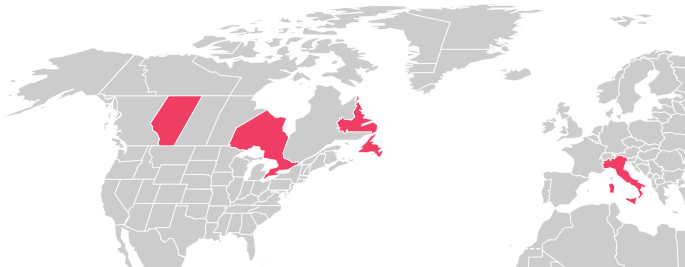
\includegraphics[scale=0.12]{img/world.png}
    ~
    ~
  \section{Top Books}
\textbf{The Innovator's Dilemma} Clayton Christensen \vspace{1.8mm}
\textbf{Lean Startup} Eric Ries \vspace{1.8mm}
\textbf{Crucial Conversations} Kerry Patterson \vspace{1.8mm}
\textbf{Rebel Talent} Francesca Gino \vspace{1.8mm}
~
%\section{Hobbies}
%\textbf{Cycling}\vspace{2mm}
%\textbf{Running}\vspace{2mm}
%\textbf{Triathlon}\vspace{2mm}
%\textbf{Opensource dev}\vspace{2mm}
%\textbf{Hardware Hacking} \vspace{2mm}
%\textbf{Deep Learning neural networks} \\ Tensorflow, Darknet neural net, Cuda \vspace{2mm}
%\textbf{Athletic performance analytics} \\ Large data analysis of public data  \vspace{2mm}
%\textbf{Sensor tech experiments} \\ strain, force, magnetic, inertial  \vspace{2mm}
\end{aside}

\section{Experience Con't}
\begin{entrylist}
%    \entry
%    {10/08 - 12/08}
%    {Maintenance Supervisor}
%    {\href{https://www.gm.ca/en/home.html}{GM Canada LTD.}}
%    {Successfully managed and maintained the paint shop maintenance department tasked with preserving the operation of conveyors, robots, and environmental control systems months before bankruptcy and restructuring.\\}
    \tentry
    {01/08 - 04/08}
    {Production Supervisor}
    {\href{https://www.gm.ca/en/home.html}{GM Canada LTD.}}
    {Consistently achieved production targets managing line workers assembling engines and wheels with less than 0.2 error rate. Awarded financial reward under Ideas for Excellence program for inventing tooling to eliminate ergonomic issues on several jobs.}{\hfill 
\includegraphics[scale=0.14]{img/GM_Canada.png}}
    \tentry
	{05/07 - 08/07}
	{Research Assistant}
	{\href{https://www.mi.mun.ca//departments/offshoresafetyandsurvivalcentreossc/}{Marine Institute OSSC}}
	{Developed a rescue prediction model using experimental data gathered during trials on the Atlantic Ocean enabling the operator of two offshore rigs to continue using only a single standby vessel when normally two are required.}
	{
\includegraphics[scale=0.05]{img/MI.png}}
	\tentry
	{09/06 - 12/06}
	{Research Assistant}
	{\href{https://www.mi.mun.ca//departments/offshoresafetyandsurvivalcentreossc/}{Marine Institute OSSC}}
	{Assisted with setup of harsh environment video capture and performed motion analysis leading to improved rescue practices for 150 person inflatable life-rafts commonly used on modern super-liners.}
	{
\includegraphics[scale=0.05]{img/MI.png}}
\end{entrylist}
\section{Education}
\begin{entrylist}
  \entry
    {2009 - 2012}
    {Master's Degree in Mechanical Engineering}
    {\href{https://www.mun.ca}{Memorial University}}
	{\textit{Development of an Active Suspension Scale Vehicle Platform}\\
Explored a new control scheme replacing expensive load cells with current sensing. Developed a dynamic test rig and validated the control scheme.}
  \entry
    {2003 - 2009}
    {Bachelor's Degree in Mechanical Engineering}
    {\href{https://www.mun.ca}{Memorial University}}
    {%
    }
\end{entrylist}
\section{Patents and Publications}
\begin{patentlist}
\pentry
    {Pedivella di Bicicletta dal lato trasmissione, dotata di rilevatore di sforzi / deformazioni per un misuratore dicoppia o di potenza, nonche' metodi correlati}
    {Bicycle Crank arm from the transmission side, equiped with strain sensors for torque or power monitoring, and related methods}    {IT102018000005302}
    \pentry
    {Rilevatore di sforzi / deformazioni per un componente di una trasmissione di bicicletta}
    {Effort sensor for a component of a bicycle transmission}
    {IT102018000005292}
    \pentry
    {Componente di bicicletta in materiale composito e relativo processo di fabbricazione}
    {Bicycle component / manufacturing process in composite material}
    {IT102018000005294}
    \pentry
    {Componente di biciletta dotato di sensore di sforzi / deformazioni compensato in temperatura }
    {Strain gage temperature compensation for bicycle component}
    {IT102018000005299}
    \pentry
    {System and method for bicycle power measurement and energy supply}
    {Application phase}
    {\href{https://patents.google.com/patent/WO2017165448A1/en}{WO2017165448A1}}
    \pentry
    {Adhesively coupled power-meter for measurement of force, torque, and power and associated methods}
    {Granted in multiple countries}
    {\href{https://patents.google.com/patent/WO2016030768A2/un}{WO2016030768A2}}
    \pentry
    {Model Complexity Requirements in Design of Half Car Active Suspension Controllers}
    {ASME 2011 Dynamic Systems and Control Conference and Bath/ASME Symposium on Fluid Power and Motion Control}
    {\href{http://proceedings.asmedigitalcollection.asme.org/proceeding.aspx?articleid=1638933}{Proceedings 2011}}
\end{patentlist}
%WO 2017165448A1 / CA 3017924 / AU 2017238156A1 \textbf{System and method for bicycle power measurement and energy supply}\\
%\emph{A crank power measurement system measures one or more of force, torque, power, and velocity of the crank, and includes a crank, two or more strain gauges located on a surface of the crank, and electronics for receiving strain data from the two or more strain gauges and determining at least one or more of bend-strain, shear-strain, and axial strain.}
%WO2016030768A2 / US 10060738B2 / EP3186590A4 / CA 2958403 / AU2015308156A1 \ \textbf{Adhesively coupled power-meter for measurement of force, torque, and power and associated methods}\\
%\emph{An adhesively coupled power-meter measures one or more of force, torque, power, and velocity of a mechanical arm}\\
%Keith J. Wakeham, Dr. D. Geoff Rideout \\
%\textbf{Model Complexity Requirements in Design of Half Car Active Suspension Controllers}\\
%\emph{This paper investigates the appropriate level of model complexity when designing optimal vehicle active suspension controllers using the Linear Quadratic Regulator (LQR) method. }
%\section{Certifications}
%\begin{entrylist}
%  \entry
%    {02/2013}
%    {Intro to Computer Science}
%    {Udacity. E-learning}
%    {\emph{Building a Python Search Engine}}
%\end{entrylist}


%\section{Other Info}
%For the Italian job market:\\
%\emph{Si autorizza il trattamento delle informazioni contenute nel curriculum in conformità alle disposizioni previste dal d.lgs. 196/2003. Si dichiara altresì di essere consapevole che, in caso di dichiarazioni non veritiere, si è passibili di sanzioni penali ai sensi del DPR 445/00 oltre alla revoca dei benefici eventualmente percepiti.}
%\begin{flushleft}
%\emph{*Note: This resume has embedded links in text}
%\end{flushleft}
\begin{flushright}
\emph{Keith Wakeham, \href{mailto:kwakeham@gmail.com}{\textbf{kwakeham@}gmail.com}}
\end{flushright}
\end{document}
